\subsection{SPI (Serial Peripheral Interface)}
\label{subsubsec:spi}
\begin{minipage}{0.48\textwidth}
Das \textit{Serial Peripheral Interface} ist ein synchrones serielles Datenprotokoll (Datenbus) bestehend aus drei Datenleitungen zur Datenübertragung. Diese sind, wie in Abbildung \ref{fig:spi} zu sehen, \textbf{MISO} (Master In Slave Out), \textbf{MOSI} (Master Out Slave In) und \textbf{SCLK} (Serial Clock). Auf dem Breakoutboard (Abb. \ref{fig:muSDBreakout}) sind die Pins mit \textbf{DI} (Data In), \textbf{DO} (Data Out) und \textbf{CLK} (Clock) beschrieben. Zu den Datenleitungen wird noch eine \textbf{SS}- (Slave Select) oder auch \textbf{CS}-Leitung (Chip Select) benötigt. Damit wird vom Master aus den zur momentanen Kommunikation nötigen Slave selektiert. Große Vorteile von SPI sind die Vollduplexfähigkeit und das Taktfrequenzen bis in den MHz-Bereich reichen. \cite{spi}\cite{Wikipedia2018spi}\\
\end{minipage}
\begin{minipage}{0.51\textwidth}
\centering
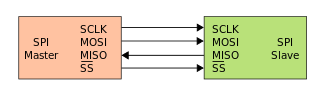
\includegraphics[width=\textwidth]{graphics/Datenspeicherung/spi_master_slave.png}
\captionof{figure}{Einfacher SPI-Datenbus \cite{Wikipedia2018spi}}
\label{fig:spi}
\end{minipage}
\todo[inline]{Möglicherweise noch die Taktfrequenz angeben, resp. die Einstellungen des SPI-Protokolls}